%%% used for replication data or other materials that do not fit the results section. Not included in 85 pages count.
\chapter*{Appendix II}
\addcontentsline{toc}{chapter}{Appendix II}


%%%%%%%%%%%%%%%%%%%%%%%%%%%%%%%%%%%%%%%%%%%%%%%%%%%%%%%%%%%%%%%%%%%%%%%%%%%%%%%% PLIP RNA
\begin{table}[H]
  \caption{\label{tab:appx2/plip} [TODO: description, for hba and hbd, pairs of atom indices are represented as A-B and separated by comma. for stacking, the rna residue numbers are provided].}
  \centering
  \begin{tabular}{ccc}
    \hline
    PDB  & interaction      & atoms / residues                                              \\ \hline
    1AKX & H-Bond Acceptors & 976-235, 975-303                                              \\
    1AKX & H-Bond Donors    & 668-969                                                       \\
    1I9V & H-Bond Acceptors & 1674-415, 1667-475, 1651-948, 1672-935, 1645-958              \\
    1I9V & H-Bond Donors    & 935-1645                                                      \\
    2ESJ & H-Bond Acceptors & 929-291, 920-323, 913-384, 915-384, 935-496, 948-496, 911-593 \\
    2ESJ & H-Bond Donors    & 404-913, 496-935, 554-924, 574-909                            \\
    4F8U & H-Bond Acceptors & 945-67, 948-82, 949-79, 944-830, 946-830                      \\
    4F8U & H-Bond Donors    & 67-945, 125-952, 145-950, 796-944, 818-944                    \\
    5BJO & H-Bond Acceptors & 1596-306, 1580-536                                            \\
    5BJO & H-Bond Donors    & 1021-1590, 305-1595                                           \\
    5BJO & Stacking         & 12, 24, 25                                                    \\
    5KX9 & H-Bond Donors    & 1017-2337, 2036-2337                                          \\
    5KX9 & Stacking         & 48, 49, 62, 85                                                \\
    6TF3 & H-Bond Donors    & 114-1135, 1001-1145, 1024-1135, 1025-1135                     \\
    6TF3 & Stacking         & 8                                                             \\
    7OAX & H-Bond Acceptors & 4696-3864, 4705-3887, 4692-3926, 4464-174                     \\
    7OAX & H-Bond Donors    & 3576-4696, 3865-4696, 159-4465, 260-4459                      \\
    7OAX & Stacking         & 14, 31                                                        \\
    8EYV & H-Bond Donors    & 1232-1993, 1448-1998                                          \\
    8EYV & Stacking         & 16, 17, 38                                                    \\ \hline
  \end{tabular}
\end{table}


%%%%%%%%%%%%%%%%%%%%%%%%%%%%%%%%%%%%%%%%%%%%%%%%%%%%%%%%%%%%%%%%%%%%%%%%%%%%%%%% STACKING POTENTIAL
\begin{figure}[H]
  \centering
  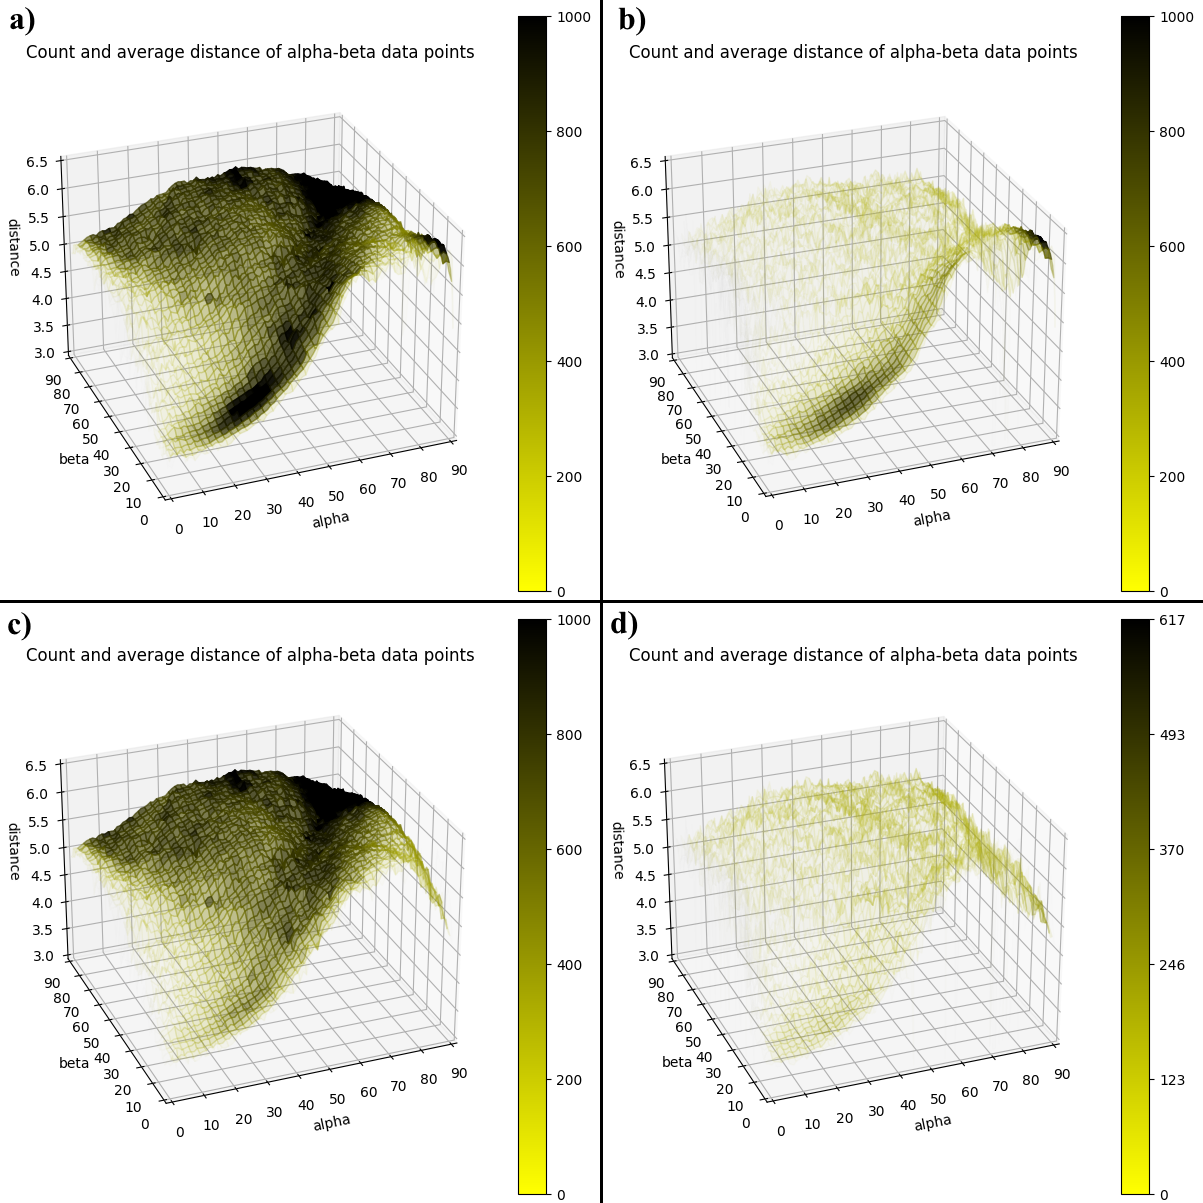
\includegraphics[width=0.7\textwidth]{figures/appendix/stacking_sampling.png}
  \caption{\label{fig:appx2/stacking_sampling} [TODO: description]}
\end{figure}


%%%%%%%%%%%%%%%%%%%%%%%%%%%%%%%%%%%%%%%%%%%%%%%%%%%%%%%%%%%%%%%%%%%%%%%%%%%%%%%% BENCHMARK PROTEIN
\begin{figure}[H]
  \centering
  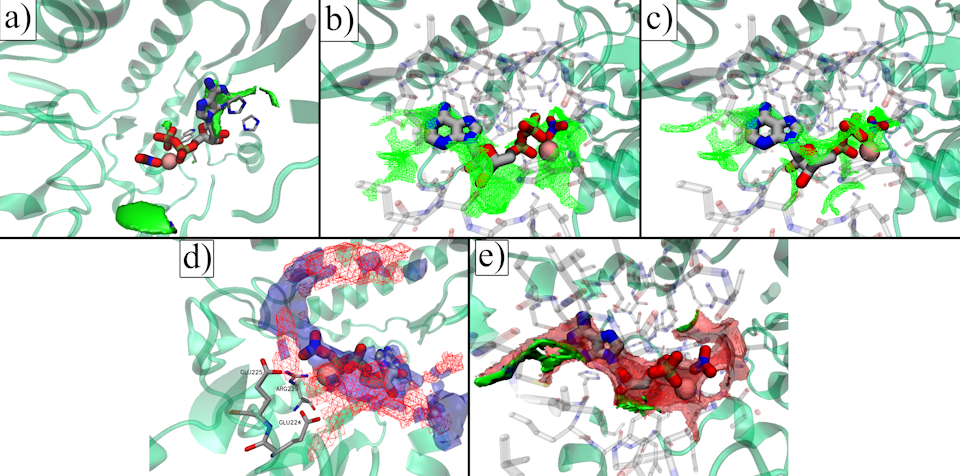
\includegraphics[width=1\textwidth]{figures/appendix/benchmark_prot/1bg0.png}
  \caption{\label{fig:appx_benchmark/1bg0} Physical properties of the pocket for the protein system PDB:1BG0. Potentials displayed: a) stacking, b) hydrogen bond acceptors, c) hydrogen bond donors, d) electrostatic, e) hydrophobicity and hydrophilicity.}
\end{figure}

\begin{figure}[H]
  \centering
  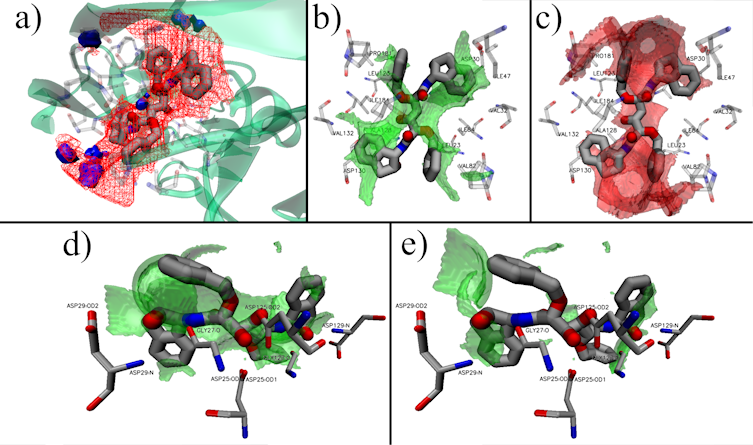
\includegraphics[width=1\textwidth]{figures/appendix/benchmark_prot/1eby.png}
  \caption{\label{fig:appx_benchmark/1eby} Physical properties of the pocket for the protein system PDB:1EBY. Potentials displayed: a) electrostatic, b) hydrophobicity, c) hydrophilicity, d) hydrogen bond acceptors, e) hydrogen bond donors.}
\end{figure}

\begin{figure}[H]
  \centering
  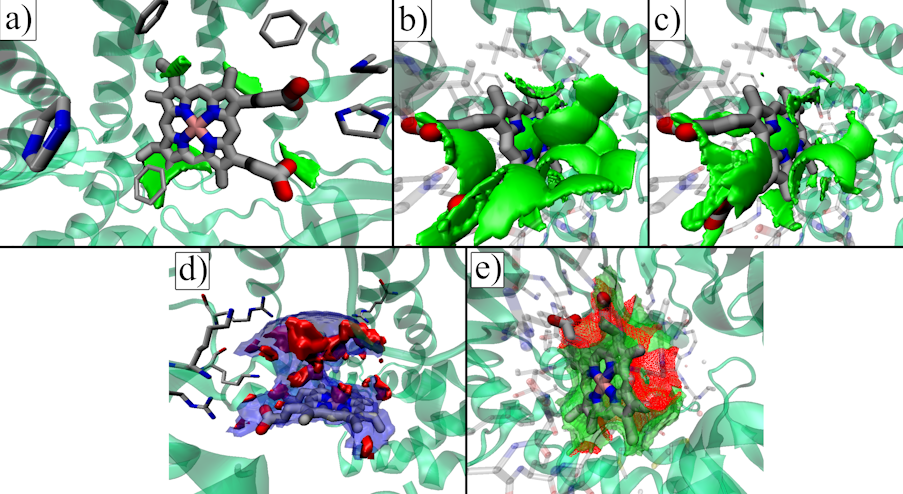
\includegraphics[width=1\textwidth]{figures/appendix/benchmark_prot/1ehe.png}
  \caption{\label{fig:appx_benchmark/1ehe} Physical properties of the pocket for the protein system PDB:1EHE. Potentials displayed: a) stacking, b) hydrogen bond acceptors, c) hydrogen bond donors, d) electrostatic, e) hydrophobicity and hydrophilicity.}
\end{figure}

\begin{figure}[H]
  \centering
  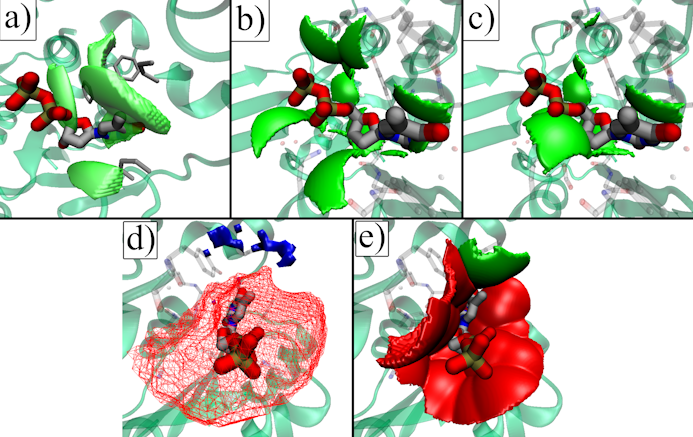
\includegraphics[width=1\textwidth]{figures/appendix/benchmark_prot/1h7l.png}
  \caption{\label{fig:appx_benchmark/1h7l} Physical properties of the pocket for the protein system PDB:1H7L. Potentials displayed: a) stacking, b) hydrogen bond acceptors, c) hydrogen bond donors, d) electrostatic, e) hydrophobicity and hydrophilicity.}
\end{figure}

\begin{figure}[H]
  \centering
  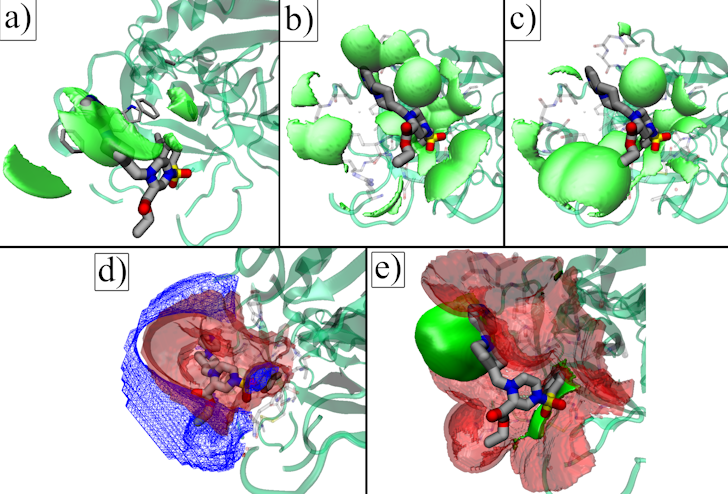
\includegraphics[width=1\textwidth]{figures/appendix/benchmark_prot/1iqj.png}
  \caption{\label{fig:appx_benchmark/1iqj} Physical properties of the pocket for the protein system PDB:1IQJ. Potentials displayed: a) stacking, b) hydrogen bond acceptors, c) hydrogen bond donors, d) electrostatic (log scale), e) hydrophobicity and hydrophilicity.}
\end{figure}

\begin{figure}[H]
  \centering
  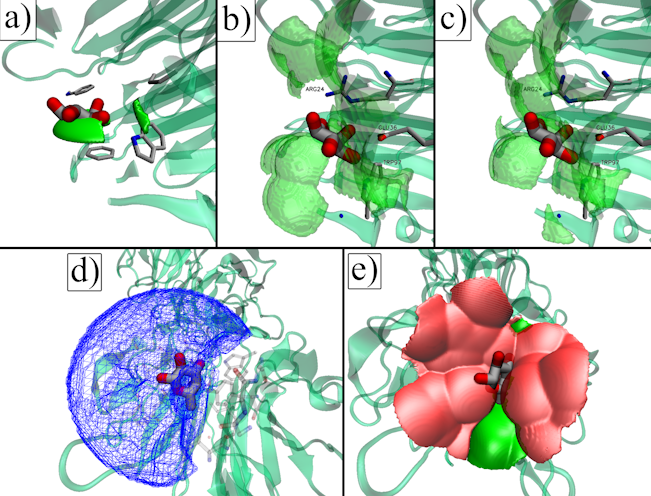
\includegraphics[width=1\textwidth]{figures/appendix/benchmark_prot/1ofz.png}
  \caption{\label{fig:appx_benchmark/1ofz} Physical properties of the pocket for the protein system PDB:1OFZ. Potentials displayed: a) stacking, b) hydrogen bond acceptors, c) hydrogen bond donors, d) electrostatic, e) hydrophobicity and hydrophilicity.}
\end{figure}

\begin{figure}[H]
  \centering
  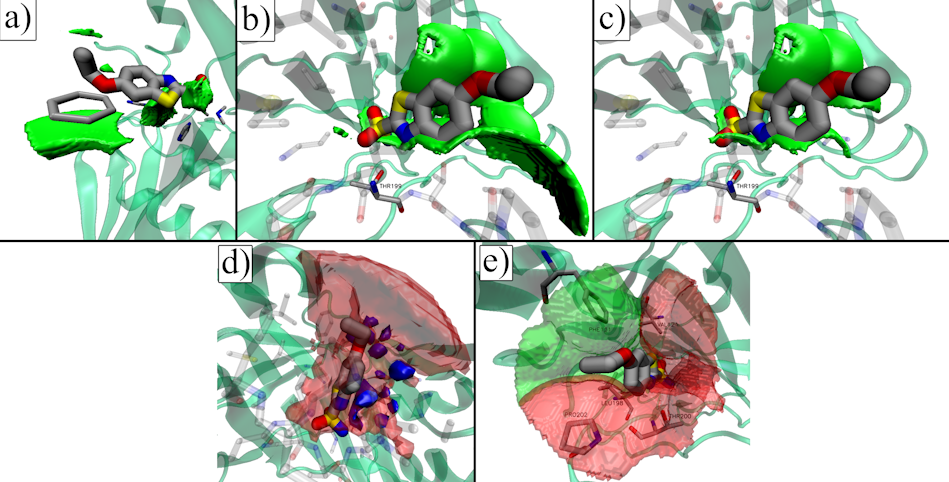
\includegraphics[width=1\textwidth]{figures/appendix/benchmark_prot/3dd0.png}
  \caption{\label{fig:appx_benchmark/3dd0} Physical properties of the pocket for the protein system PDB:3DD0. Potentials displayed: a) stacking, b) hydrogen bond acceptors, c) hydrogen bond donors, d) electrostatic, e) hydrophobicity and hydrophilicity.}
\end{figure}

\begin{figure}[H]
  \centering
  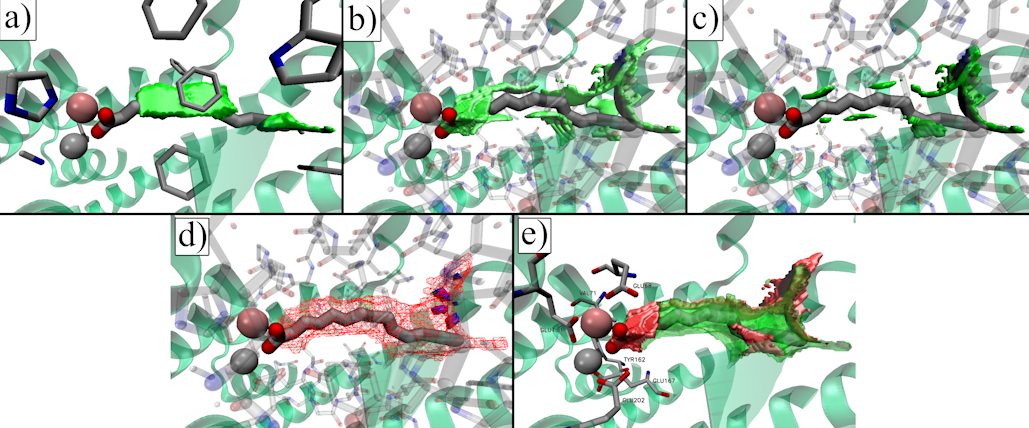
\includegraphics[width=1\textwidth]{figures/appendix/benchmark_prot/3ee4.png}
  \caption{\label{fig:appx_benchmark/3ee4} Physical properties of the pocket for the protein system PDB:3EE4. Potentials displayed: a) stacking, b) hydrogen bond acceptors, c) hydrogen bond donors, d) electrostatic, e) hydrophobicity and hydrophilicity.}
\end{figure}

\begin{figure}[H]
  \centering
  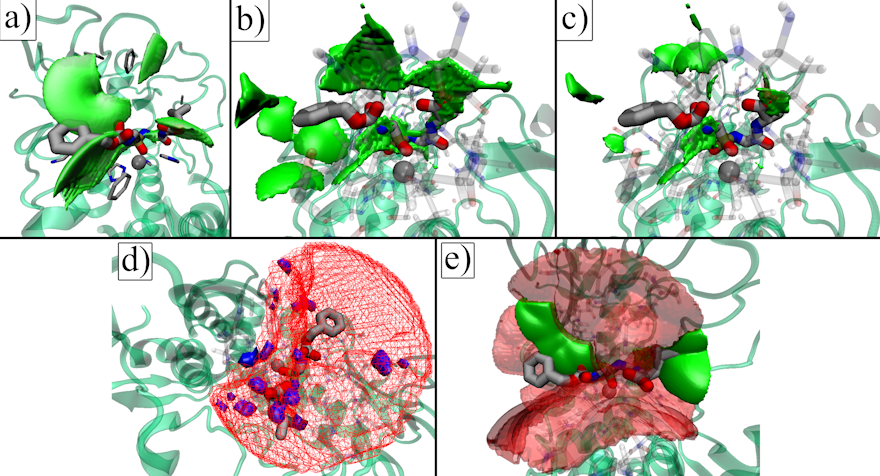
\includegraphics[width=1\textwidth]{figures/appendix/benchmark_prot/5m9w.png}
  \caption{\label{fig:appx_benchmark/5m9w} Physical properties of the pocket for the protein system PDB:5M9W. Potentials displayed: a) stacking, b) hydrogen bond acceptors, c) hydrogen bond donors, d) electrostatic, e) hydrophobicity and hydrophilicity.}
\end{figure}

\begin{figure}[H]
  \centering
  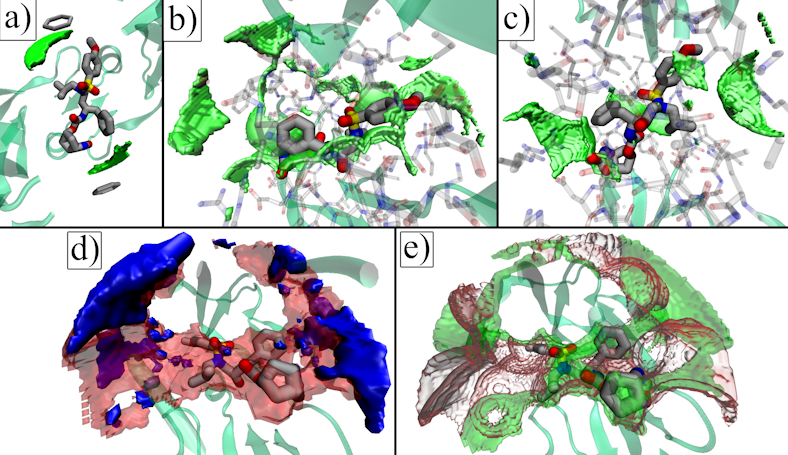
\includegraphics[width=1\textwidth]{figures/appendix/benchmark_prot/6e9a.png}
  \caption{\label{fig:appx_benchmark/6e9a} Physical properties of the pocket for the protein system PDB:6E9A. Potentials displayed: a) stacking, b) hydrogen bond acceptors, c) hydrogen bond donors, d) electrostatic (log scale), e) hydrophobicity and hydrophilicity.}
\end{figure}

%%%%%%%%%%%%%%%%%%%%%%%%%%%%%%%%%%%%%%%%%%%%%%%%%%%%%%%%%%%%%%%%%%%%%%%%%%%%%%%% BENCHMARK RNA
\begin{figure}[H]
  \centering
  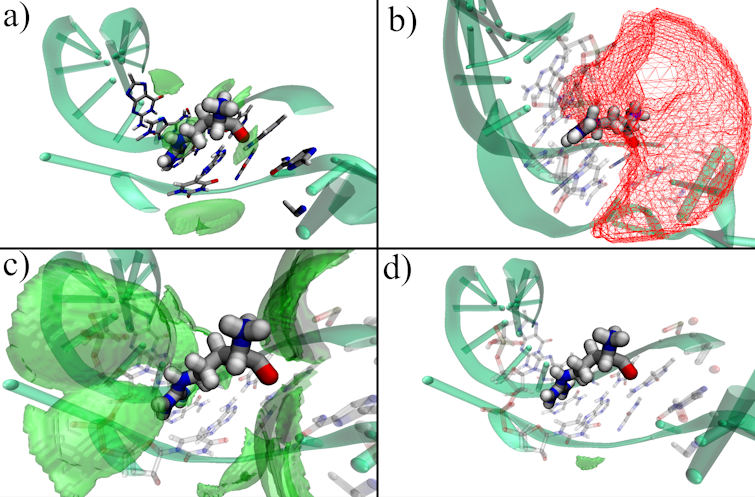
\includegraphics[width=0.8\textwidth]{figures/appendix/benchmark_rna/1akx.png}
  \caption{\label{fig:appx_benchmark/1akx} Physical properties of the pocket for the RNA system PDB:1AKX. Potentials displayed: a) stacking, b) electrostatic, c) hydrogen bond acceptors, d) hydrogen bond donors.}
\end{figure}

\begin{figure}[H]
  \centering
  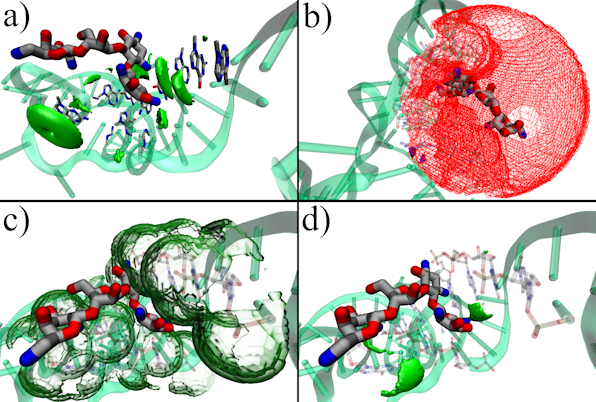
\includegraphics[width=0.8\textwidth]{figures/appendix/benchmark_rna/1i9v.png}
  \caption{\label{fig:appx_benchmark/1i9v} Physical properties of the pocket for the RNA system PDB:1I9V. Potentials displayed: a) stacking, b) electrostatic, c) hydrogen bond acceptors, d) hydrogen bond donors.}
\end{figure}

\begin{figure}[H]
  \centering
  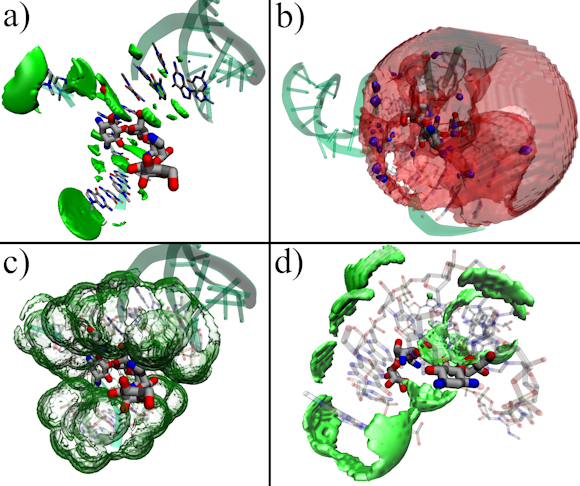
\includegraphics[width=0.8\textwidth]{figures/appendix/benchmark_rna/2esj.png}
  \caption{\label{fig:appx_benchmark/2esj} Physical properties of the pocket for the RNA system PDB:2ESJ. Potentials displayed: a) stacking, b) electrostatic, c) hydrogen bond acceptors, d) hydrogen bond donors.}
\end{figure}

\begin{figure}[H]
  \centering
  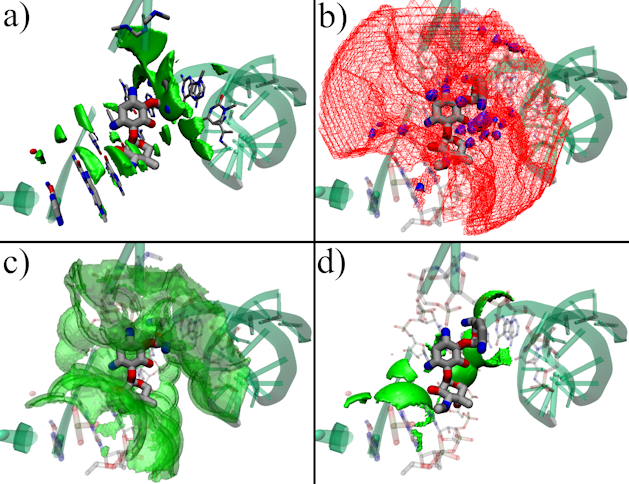
\includegraphics[width=0.8\textwidth]{figures/appendix/benchmark_rna/4f8u.png}
  \caption{\label{fig:appx_benchmark/4f8u} Physical properties of the pocket for the RNA system PDB:4F8U. Potentials displayed: a) stacking, b) electrostatic, c) hydrogen bond acceptors, d) hydrogen bond donors.}
\end{figure}

\begin{figure}[H]
  \centering
  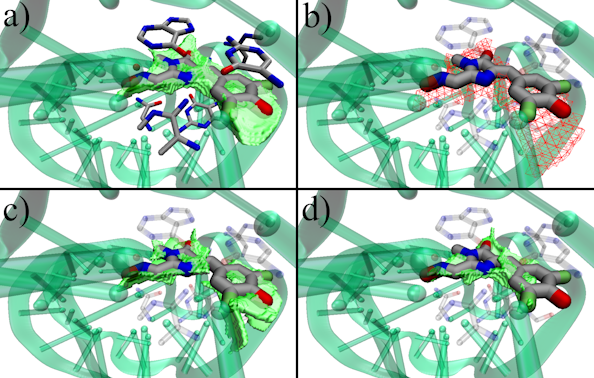
\includegraphics[width=0.8\textwidth]{figures/appendix/benchmark_rna/5bjo.png}
  \caption{\label{fig:appx_benchmark/5bjo} Physical properties of the pocket for the RNA system PDB:5BJO. Potentials displayed: a) stacking, b) electrostatic, c) hydrogen bond acceptors, d) hydrogen bond donors.}
\end{figure}

\begin{figure}[H]
  \centering
  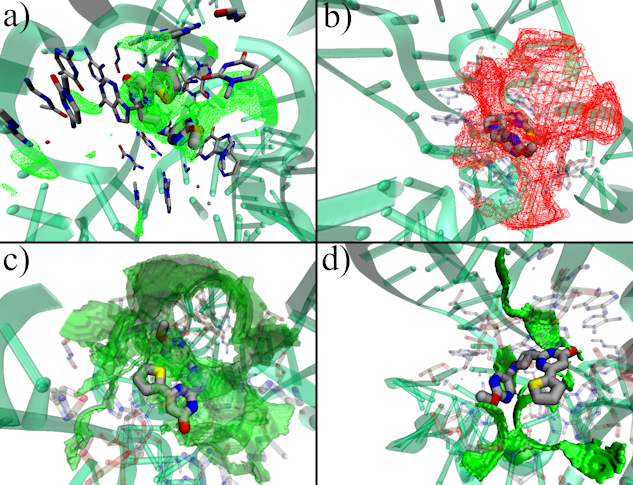
\includegraphics[width=0.8\textwidth]{figures/appendix/benchmark_rna/5kx9.png}
  \caption{\label{fig:appx_benchmark/5kx9} Physical properties of the pocket for the RNA system PDB:5KX9. Potentials displayed: a) stacking, b) electrostatic, c) hydrogen bond acceptors, d) hydrogen bond donors.}
\end{figure}

\begin{figure}[H]
  \centering
  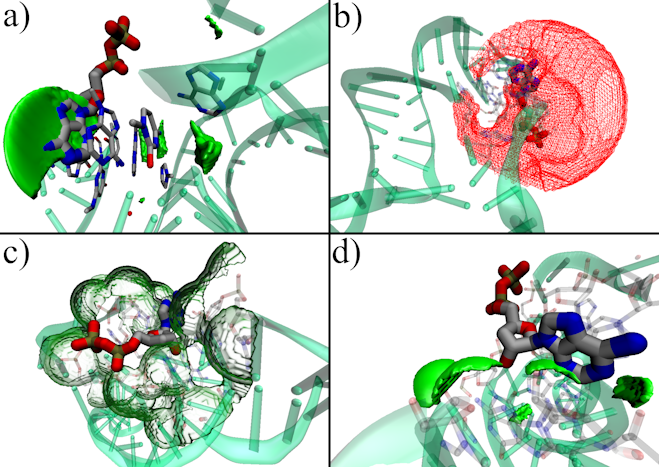
\includegraphics[width=0.8\textwidth]{figures/appendix/benchmark_rna/6tf3.png}
  \caption{\label{fig:appx_benchmark/6tf3} Physical properties of the pocket for the RNA system PDB:6TF3. Potentials displayed: a) stacking, b) electrostatic, c) hydrogen bond acceptors, d) hydrogen bond donors.}
\end{figure}

\begin{figure}[H]
  \centering
  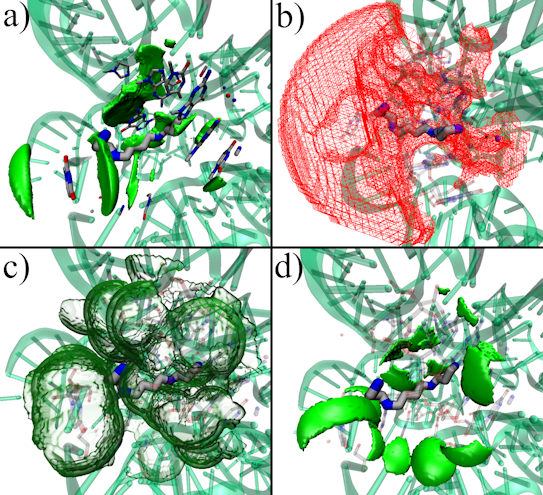
\includegraphics[width=0.8\textwidth]{figures/appendix/benchmark_rna/7oax0.png}
  \caption{\label{fig:appx_benchmark/7oax0} Physical properties of the pocket for the RNA system PDB:7OAX (ligand: SPM). Potentials displayed: a) stacking, b) electrostatic, c) hydrogen bond acceptors, d) hydrogen bond donors.}
\end{figure}

\begin{figure}[H]
  \centering
  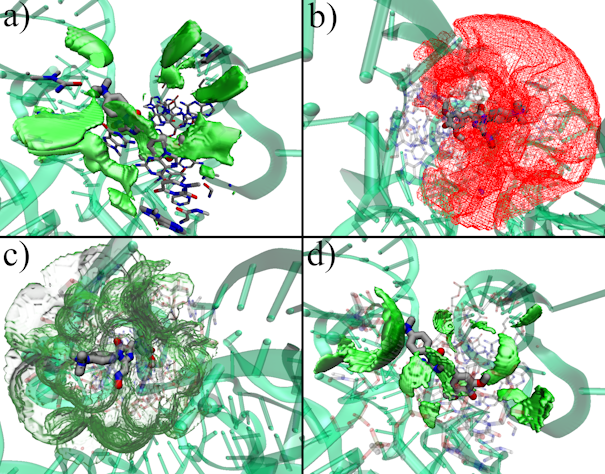
\includegraphics[width=0.8\textwidth]{figures/appendix/benchmark_rna/7oax1.png}
  \caption{\label{fig:appx_benchmark/7oax1} Physical properties of the pocket for the RNA system PDB:7OAX (ligand: V5Z). Potentials displayed: a) stacking, b) electrostatic, c) hydrogen bond acceptors, d) hydrogen bond donors.}
\end{figure}

\begin{figure}[H]
  \centering
  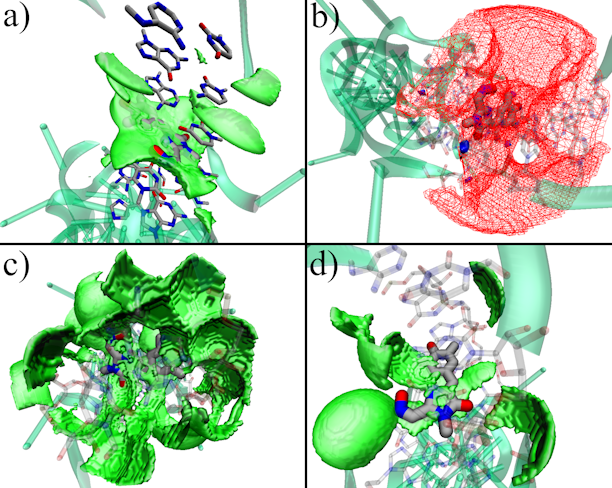
\includegraphics[width=0.8\textwidth]{figures/appendix/benchmark_rna/8eyv.png}
  \caption{\label{fig:appx_benchmark/8eyv} Physical properties of the pocket for the RNA system PDB:8EYV. Potentials displayed: a) stacking, b) electrostatic, c) hydrogen bond acceptors, d) hydrogen bond donors.}
\end{figure}


%%%%%%%%%%%%%%%%%%%%%%%%%%%%%%%%%%%%%%%%%%%%%%%%%%%%%%%%%%%%%%%%%%%%%%%%%%%%%%%%
